% Copyright (c) 2015 Jeremie DECOCK (http://www.jdhp.org)

% This document is provided under the terms of the "Creative Commons BY-SA" license.
% For more details, read the "COPYING/legalcode.html" enclosed file or
% the "http://creativecommons.org/licenses/by-sa/4.0/legalcode" web page.

\documentclass{article}

\usepackage[utf8]{inputenc}
\usepackage[T1]{fontenc}

% English environment
%\usepackage[english]{babel}

% French environment
\usepackage[french]{babel}

% French + English environment
%\usepackage[francais,english]{babel}

%%%%%%%%%%%%%%%%%%%%%%%%%%%%%%%%%%%%%%%%%%%%%%%%%%%%%%%%%%%%%%%%%%%%%%%%%%%%%%%%

% Clickable Table of Contents
% http://tex.stackexchange.com/questions/73862/how-can-i-make-a-clickable-table-of-contents
\usepackage{hyperref}
\hypersetup{
	pdftoolbar=true,                                          % show Acrobat’s toolbar ?
	pdfmenubar=true,                                          % show Acrobat’s menu ?
	pdffitwindow=true,                                        % page fit to window when opened
	pdfnewwindow=true,                                        % links in new window
	colorlinks=true,                                          % false: boxed links; true: colored links
	linkcolor=black,                                          % color of internal links
	citecolor=black,                                          % color of links to bibliography
	filecolor=black,                                          % color of file links
	urlcolor=black                                            % color of external links
}

\usepackage{algorithm}
\usepackage{algorithmic}
\usepackage{amsmath}
\usepackage{amssymb}
%\usepackage{bm}    % bold math
\usepackage{color}  % change text color
\usepackage{xcolor} % required for listings package...
\usepackage{epsfig}
\usepackage{eurosym}
\usepackage{flushend}
\usepackage{graphicx}
\usepackage{ifthen}
\usepackage{multirow}
%\usepackage{natbib} % For bibliography, often used nowadays
\usepackage{subfigure}
\usepackage{url}

%% Inserting a pdf file in the document
%% See: http://stackoverflow.com/questions/2739159/inserting-a-pdf-file-in-latex 
%\usepackage{pdfpages}
%\usepackage{epsfig}
%\usepackage{geometry}
%\usepackage{pdflscape}

%%%%%%%%%%%%%%%%%%%%%%%%%%%%%%%%%%%%%%%%%%%%%%%%%%%%%%%%%%%%%%%%%%%%%%%%%%%%%%%%

%\usepackage[font=sf, labelfont={sf,bf}, margin=1cm]{caption}
%\usepackage[font=rm, margin=1cm]{caption}

% HeVeA %%%%%%%%%%%%%%%%%%%%%%%%%%%%%%%%%%%%%%%%%%%%%%%%%%%%%%%%%%%%%%%%%%%%%%%

\usepackage{hevea}
\newstyle{body}{margin-left: auto; margin-right: auto; padding: .5em 1.5em; max-width: 50em; text-align: justify; font-family: sans-serif;}
\newstyle{div.lstlisting}{font-size: 130\%; margin-left: auto; margin-right: auto; width: 35em;}

\newif\ifpdf                   
\ifx\pdfoutput\undefined
\pdffalse
\else
\pdfoutput=1
\pdftrue
\fi

% TikZ %%%%%%%%%%%%%%%%%%%%%%%%%%%%%%%%%%%%%%%%%%%%%%%%%%%%%%%%%%%%%%%%%%%%%%%%

%\usepackage{tikz}
%\input{setup_package_tikz.tex}

% Listings package settings %%%%%%%%%%%%%%%%%%%%%%%%%%%%%%%%%%%%%%%%%%%%%%%%%%%%

%\usepackage{listings}
%\input{setup_package_listings.tex}


%% COMMANDS AND DEFS %%%%%%%%%%%%%%%%%%%%%%%%%%%%%%%%%%%%%%%%%%%%%%%%%%%%%%%%%%%

% Pour désactiver temporairement les images (compile beaucoup plus vite)
%\renewcommand{\includegraphics}[2][]{\null}

%%% Math symbols

%\renewcommand{\vec}[1]{\ensuremath{\boldsymbol{#1}}} % bold vectors
\newcommand{\vs}[1]{\boldsymbol{#1}} % vector symbol (\boldsymbol, \textbf or \vec)
\newcommand{\ms}[1]{\boldsymbol{#1}} % matrix symbol (\boldsymbol, \textbf)

\newcommand{\x}{\vs{x}}
\newcommand{\xstar}{\vs{x^*}}
\newcommand{\w}{\vs{\omega}}
\newcommand{\objfunc}{f}

\def\bbbr{{\rm I\!R}} % reelle Zahlen

\newcommand{\E}{\mathbb{E}}
\newcommand{\N}{\mathbb{N}}
\newcommand{\Z}{\mathbb{Z}}
\newcommand{\Q}{\mathbb{Q}}
\newcommand{\R}{{\bbbr}{}}
\newcommand{\C}{\mathbb{C}}
\newcommand{\K}{\mathbb{K}}

\newcommand{\mb}[1]{\mathbb{#1}}
\newcommand{\mc}[1]{\mathcal{#1}}

\def\CQFD{\fbox\\}

%%% General commands

\newenvironment{jmatrix}{\renewcommand\arraystretch{1.5} \begin{pmatrix}}{\end{pmatrix}}
%\renewcommand{\arraystretch}{1.5}

\newcommand{\cred}[1]{\textcolor{red}{#1}}
\newcommand{\ech}[1]{\textcolor{gray}{#1}}
\newcommand{\imp}[1]{{\em {#1}}}
\newcommand{\voc}[1]{{\em {#1}}}
\newcommand{\todo}[1][\dots]{\textbf{[TODO : #1]}}  % todo mark

\newcommand{\dontforget}[1]{\textcolor{red}{#1}}

\newcommand{\HRule}{\rule{\linewidth}{0.5mm}}

%%% Debug: Display the current table counter (cf. http://www.iam.ubc.ca/old_pages/newbury/tex/numbering.html)

\newcommand{\tablecounterdebug}{\textbf{Table~counter:~\thetable}\\}
\newcommand{\equationcounterdebug}{\textbf{Equation~counter:~\theequation}\\}
\newcommand{\figurecounterdebug}{\textbf{Figure~counter:~\thefigure}\\}
\newcommand{\algorithmcounterdebug}{\textbf{Algorithm~counter:~\thealgorithm}\\}



\sloppy

%%%%%%%%%%%%%%%%%%%%%%%%%%%%%%%%%%%%%%%%%%%%%%%%%%%%%%%%%%%%%%%%%%%%%%%%%%%%%%%

\title{Accéder à la mémoire des appareils Android sur Debian Jessie via le protocole MTP}

\author{Jérémie \textsc{Decock} \\ \url{http://www.jdhp.org}}

%\institute{ \textsuperscript{1}TAO, INRIA-CNRS-LRI, Univ. Paris-Sud, 91190 Gif-sur-Yvette, France}
\date{24 janvier 2015}

\hypersetup{
	pdftitle={Accéder à la mémoire des appareils Android sur Debian Jessie via le protocole MTP},     % title
	pdfauthor={Jérémie DECOCK},      % author
	pdfsubject={Accéder à la mémoire des appareils Android sur Debian Jessie via le protocole MTP}, % subject of the document
	pdfkeywords={mtp, debian, android}         % list of keywords
}

%%%%%%%%%%%%%%%%%%%%%%%%%%%%%%%%%%%%%%%%%%%%%%%%%%%%%%%%%%%%%%%%%%%%%%%%%%%%%%%

\begin{document}

\maketitle

%\tableofcontents

% Introduction %%%%%%%%%%%%%%%%%%%%%%%%%%%%%%%%%%%%%%%%%%%%%%%%%%%%%%%%%%%%%%%%

\section*{Introduction}\label{sec:intro}

Ce tutoriel très court décrit simplement comment accéder à la mémoire
des téléphones et tablettes Android sur Debian Jessie.

Ici on ne suppose pas d'environnement de bureau particulier~; les
opérations décrites dans la suite de ce tutoriel sont effectuées depuis un
terminal.

Les appareils Android récents (versions 4 et plus) utilisent le protocole
\href{http://fr.wikipedia.org/wiki/Media_Transfer_Protocol}{MTP} pour partager
le contenu de leurs cartes mémoire avec un ordinateur, au détriment du
protocole {\em USB Mass Storage} utilisé jusque là sur ce type d'appareils.
MTP (Media Transfer Protocol) est un protocole développé par Microsoft pour
permettre l'échange de données avec les appareils multimédia mobiles (appareils
photo, lecteurs MP3, ...).
Jusqu'à récemment, ce protocole était mal géré et mal intégré dans les
systèmes Gnu/Linux. Plusieurs solutions se sont succédées pour accéder avec plus ou
moins de succès aux mémoires des appareils Android.
Une des solutions les plus souvent évoquées sur Internet est {\em go-mtpfs},
un système de fichier
\href{http://fr.wikipedia.org/wiki/Filesystem_in_Userspace}{FUSE} qui permet le
montage des périphériques MTP.
Go-mtpfs n'est malheureusement pas disponible dans les dépôts officiels de
Debian~; c'est pourquoi je vais présenter ici une autre solution, qui m'a donné
entière satisfaction~: {\em jmtpfs}.

Jmtpfs est un autre système de fichier FUSE. Il est intégré dans
les dépôts officiels de Debian Jessie et a la réputation d'être assez stable.
Pour pouvoir l'utiliser, il suffit d'installer le paquet {\em jmtpfs}~:
\begin{verbatim}
# apt-get install jmtpfs
\end{verbatim}

% Section 1 %%%%%%%%%%%%%%%%%%%%%%%%%%%%%%%%%%%%%%%%%%%%%%%%%%%%%%%%%%%%%%%%%%%

\section*{Accéder aux données}\label{sec:intall-qemu}

Une fois l'appareil Android branché à l'ordinateur via le port USB,
on peut monter son volume de données dans le répertoire
\textasciitilde{}/mtp (par exemple) via la commande suivante~:
\begin{verbatim}
$ jmtpfs ~/mtp
\end{verbatim}

Le contenu de l'appareil Android est alors accessible en lecture et en écriture
dans le répertoire \textasciitilde{}/mtp.

Attention, de nombreux appareils Android nécessitent une confirmation ou un
déblocage avant le premier accès aux données via MTP.

Si plusieurs appareils compatibles MTP sont branchés sur l'ordinateur, il faut
spécifier l'appareil à monter avec l'option {\em -device}~:

\begin{verbatim}
$ jmtpfs -device=<busnum>,<devnum> ~/mtp
\end{verbatim}

Les identifiants {\em <busnum>} et {\em <devnum>} peuvent être obtenus avec la
commande suivante~:
\begin{verbatim}
$ jmtpfs -l
\end{verbatim}

Une fois les transferts de fichier opérés, on peut démonter le volume avec la
commande~:
\begin{verbatim}
$ fusermount -u ~/mtp
\end{verbatim}

Il arrive que l'appareil Android ne réponde pas, ce qui peut bloquer les
processus qui tentent d'accéder au point de montage sur l'ordinateur.
Une solution dans ce cas, est de forcer le démontage du volume avec l'option
{\em -z}~:
\begin{verbatim}
$ fusermount -uz ~/mtp
\end{verbatim}

% Section CCL %%%%%%%%%%%%%%%%%%%%%%%%%%%%%%%%%%%%%%%%%%%%%%%%%%%%%%%%%%%%%%%%%

%\section*{Conclusion}\label{sec:ccl}


% Bibliography %%%%%%%%%%%%%%%%%%%%%%%%%%%%%%%%%%%%%%%%%%%%%%%%%%%%%%%%%%%%%%%%

%\nocite{decock:hal-00755663}  % fait apparaitre le document dans la bibliographie sans le citer !
\nocite{*}                    % fait apparaitre TOUS les documents du .bib dans la bibliographie sans les citer !

\bibliographystyle{plain}    % name of the .bst file (bibliography style)
\bibliography{bibliography}  % name of the .bib file (without the file name extension)


% Section License %%%%%%%%%%%%%%%%%%%%%%%%%%%%%%%%%%%%%%%%%%%%%%%%%%%%%%%%%%%%%

\ifpdf
    \vfill % Go to the bottom of the page...
    \begin{center}
        \href{http://creativecommons.org/licenses/by-sa/4.0/}{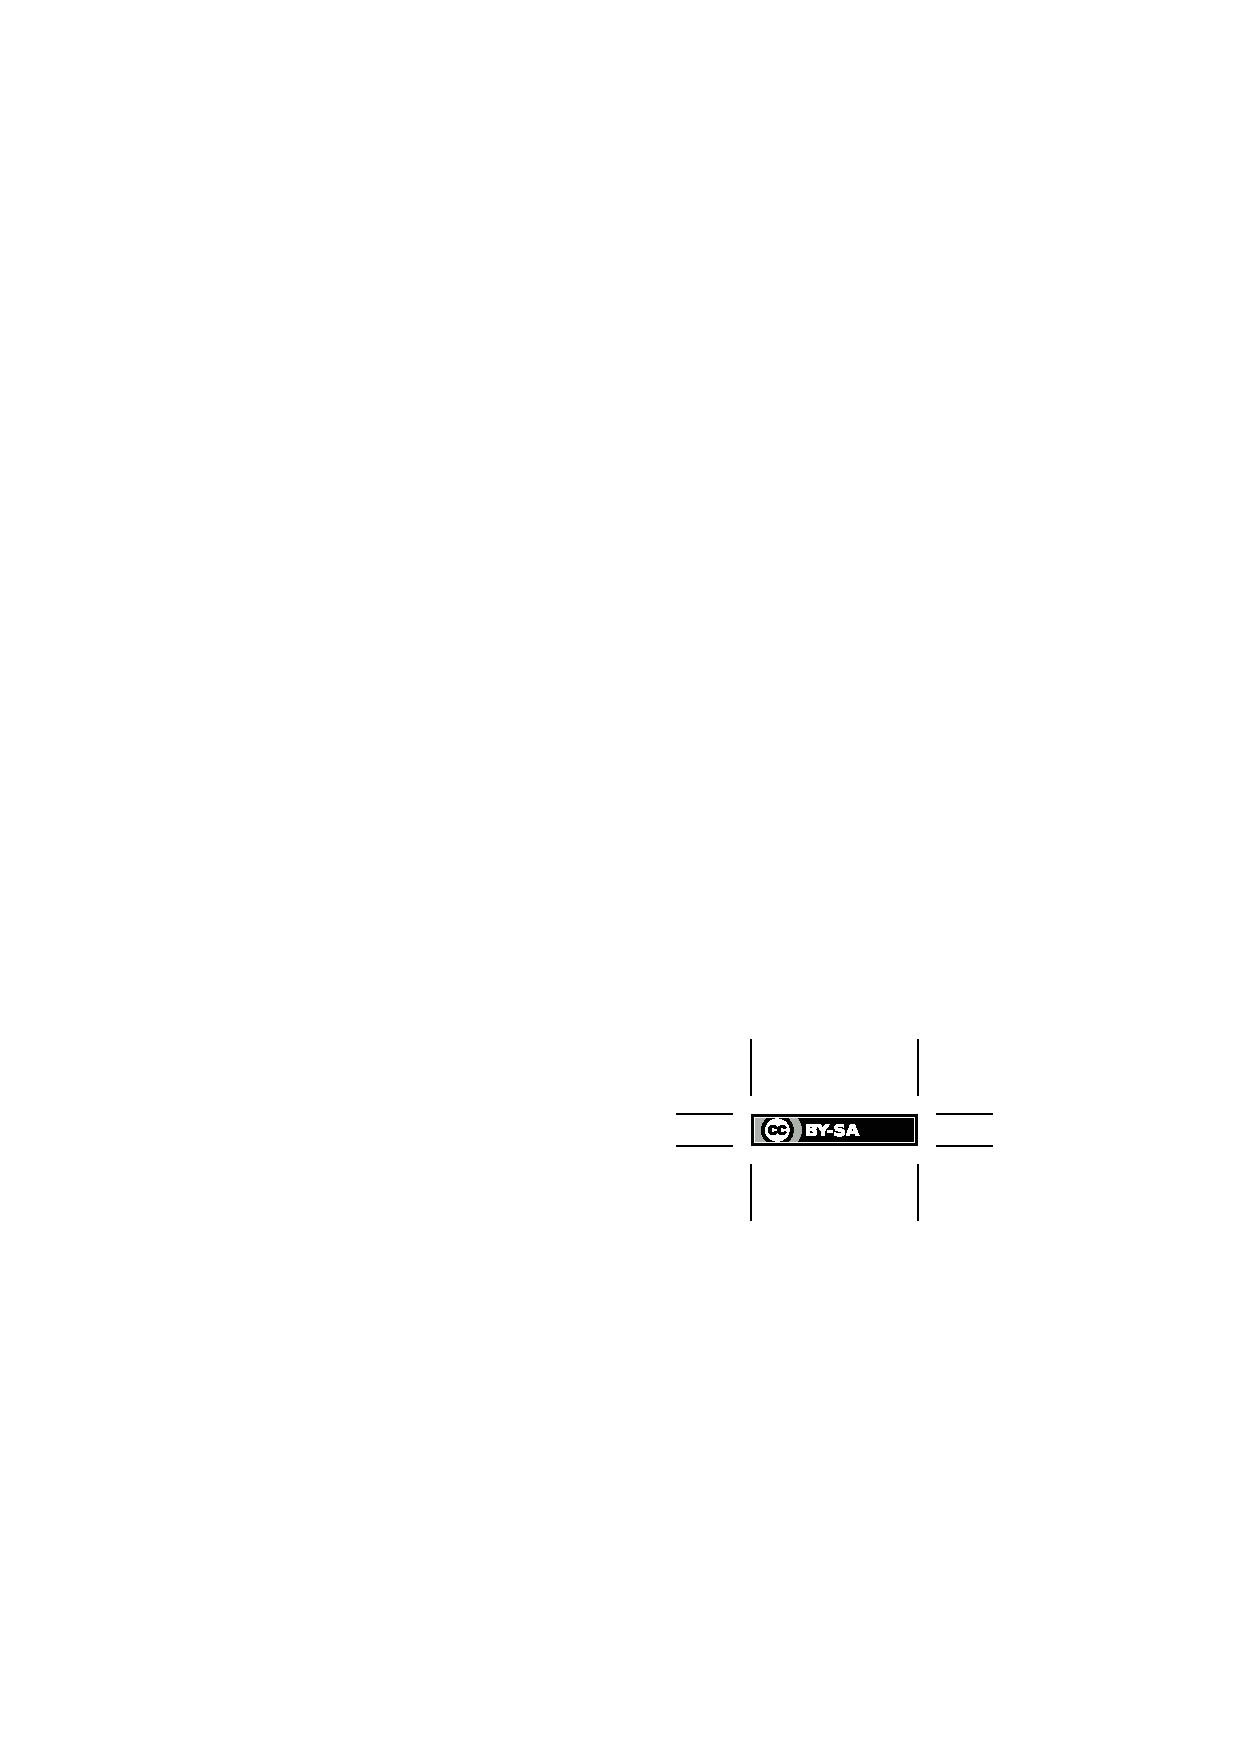
\includegraphics[width=.15\linewidth]{fig/cc_by_sa_small}}\\
        \small{Creative Commons BY-SA}
    \end{center}
\else
    % HeVeA
    \section*{License}\label{sec:license}

    \begin{rawhtml}

        <div>
            <a rel="license" href="http://creativecommons.org/licenses/by-sa/4.0/">
                <img alt="Licence Creative Commons" style="border-width:0" src="https://i.creativecommons.org/l/by-sa/4.0/80x15.png" />
            </a>
            <br />
            <span xmlns:dct="http://purl.org/dc/terms/" href="http://purl.org/dc/dcmitype/Text" property="dct:title" rel="dct:type"><em>Accéder à la mémoire des appareils Android sur Debian Jessie via le protocole MTP</em></span> de <a xmlns:cc="http://creativecommons.org/ns#" href="http://www.jdhp.org" property="cc:attributionName" rel="cc:attributionURL">Jérémie Decock</a> est mis à disposition selon les termes de la <a rel="license" href="http://creativecommons.org/licenses/by-sa/4.0/">licence Creative Commons Attribution -  Partage dans les Mêmes Conditions 4.0 International</a>.
        </div>

    \end{rawhtml}
\fi

\end{document}
